\section{ImageLocate}\label{sec:imagelocate}
\fontsize{12}{12}\selectfont
    \par A função ImageLocateSubImage() é usada para determinar se a imagem2 é uma parte da imagem1.
        Para esta função funcionar corretamente, esta chama a função ImageMatchSubImage() para comparar os pixeis 
        de modo a garantir que a imagem2 é, de facto, igual a uma parte da imagem1.

\subsection{Eficiência computacional da ImageLocateSubImage()}
    \par Para analisar a sua eficiência computacional, foi registado numa tabela \autoref{tab:locate} o 
    número de comparações envolvendo uma sequência de testes com diferentes imagens. 

\begin{center}
    \begin{table}[h]
        \centering
        \begin{tabular}{| p{2cm} | p{3cm} | p{1.5cm} | p{2cm} | p{5cm} |}
        \hline
        \textbf{Img1} & \textbf{Img2} & \textbf{Iterações da Locate} & \textbf{Iterações da Match} & \textbf{Observações} \\ \hline
        original.pgm (300x300) & crop.pgm (100x100) & 3010 & 10000 & \\ \hline
        original.pgm (300x300) & rotate.pgm (300x300) & 90000 & 90000 & 
            img2 doesn't fit if it starts at another pixel other than (0,0) in img1 \\ \hline
        ireland.pgm (1600x1200) & airfield (1600x1200) & 1920000 & 1920000 &
            img2 doesn't fit in img1, if it starts in a different ixel than (0,0)  \\ \hline
        airfield (1600x1200) & ireland (640x480) & 1920000 & 1 &
            first pixel of img2 is different than img1, so the loop is only executed one time \\ \hline
        airfield (1600x1200) & airfieldCrop (100x100) & 1 & 10000 &  \\ \hline
        airfield (1600x1200) & airfieldCrop (10x10)  & 1 & 100 & \\ \hline
        airfield (1600x1200) & airfieldCrop (10x10) (no ponto 1549,1189) & 1903950 & 1898830 & \\ \hline                 
        \end{tabular}
        \caption{Tabela com dados resultantes das iterações da função ImageLocateSubImage() e ImageMatchSubImage()}
        \label{tab:locate}
    \end{table}
\end{center}

\newpage 

\begin{itemize}
    \item \textbf{Best Case:} Imagens com pouca resolução e a imagem2 está localizada no pixel (0,0)
    \item \textbf{Average case:} Imagem tem pouca resolução e a imagem2 não se encontra localizada nela
    \item \textbf{Worst case:} Imagens com grande resolução e a imagem 2 não se encontra localizada nela
        ou a imagem2 é uma porção pequena do canto inferior direito da imagem2
\end{itemize}

\subsection{Funcionamento da ImageLocateSubImage()}
    \par Este algoritmo segue uma lógica básica por detrás. Sâo enviadas duas imagens, img1 e img2, e é feita 
        a comparação entre os pixeis da img1 e da img2, sendo o ínicio no pixel (0,0) até ao pixel ($width,$height),
        tal como consta na \autoref{fig:locate}.

    \begin{figure} [H]
        \centering
        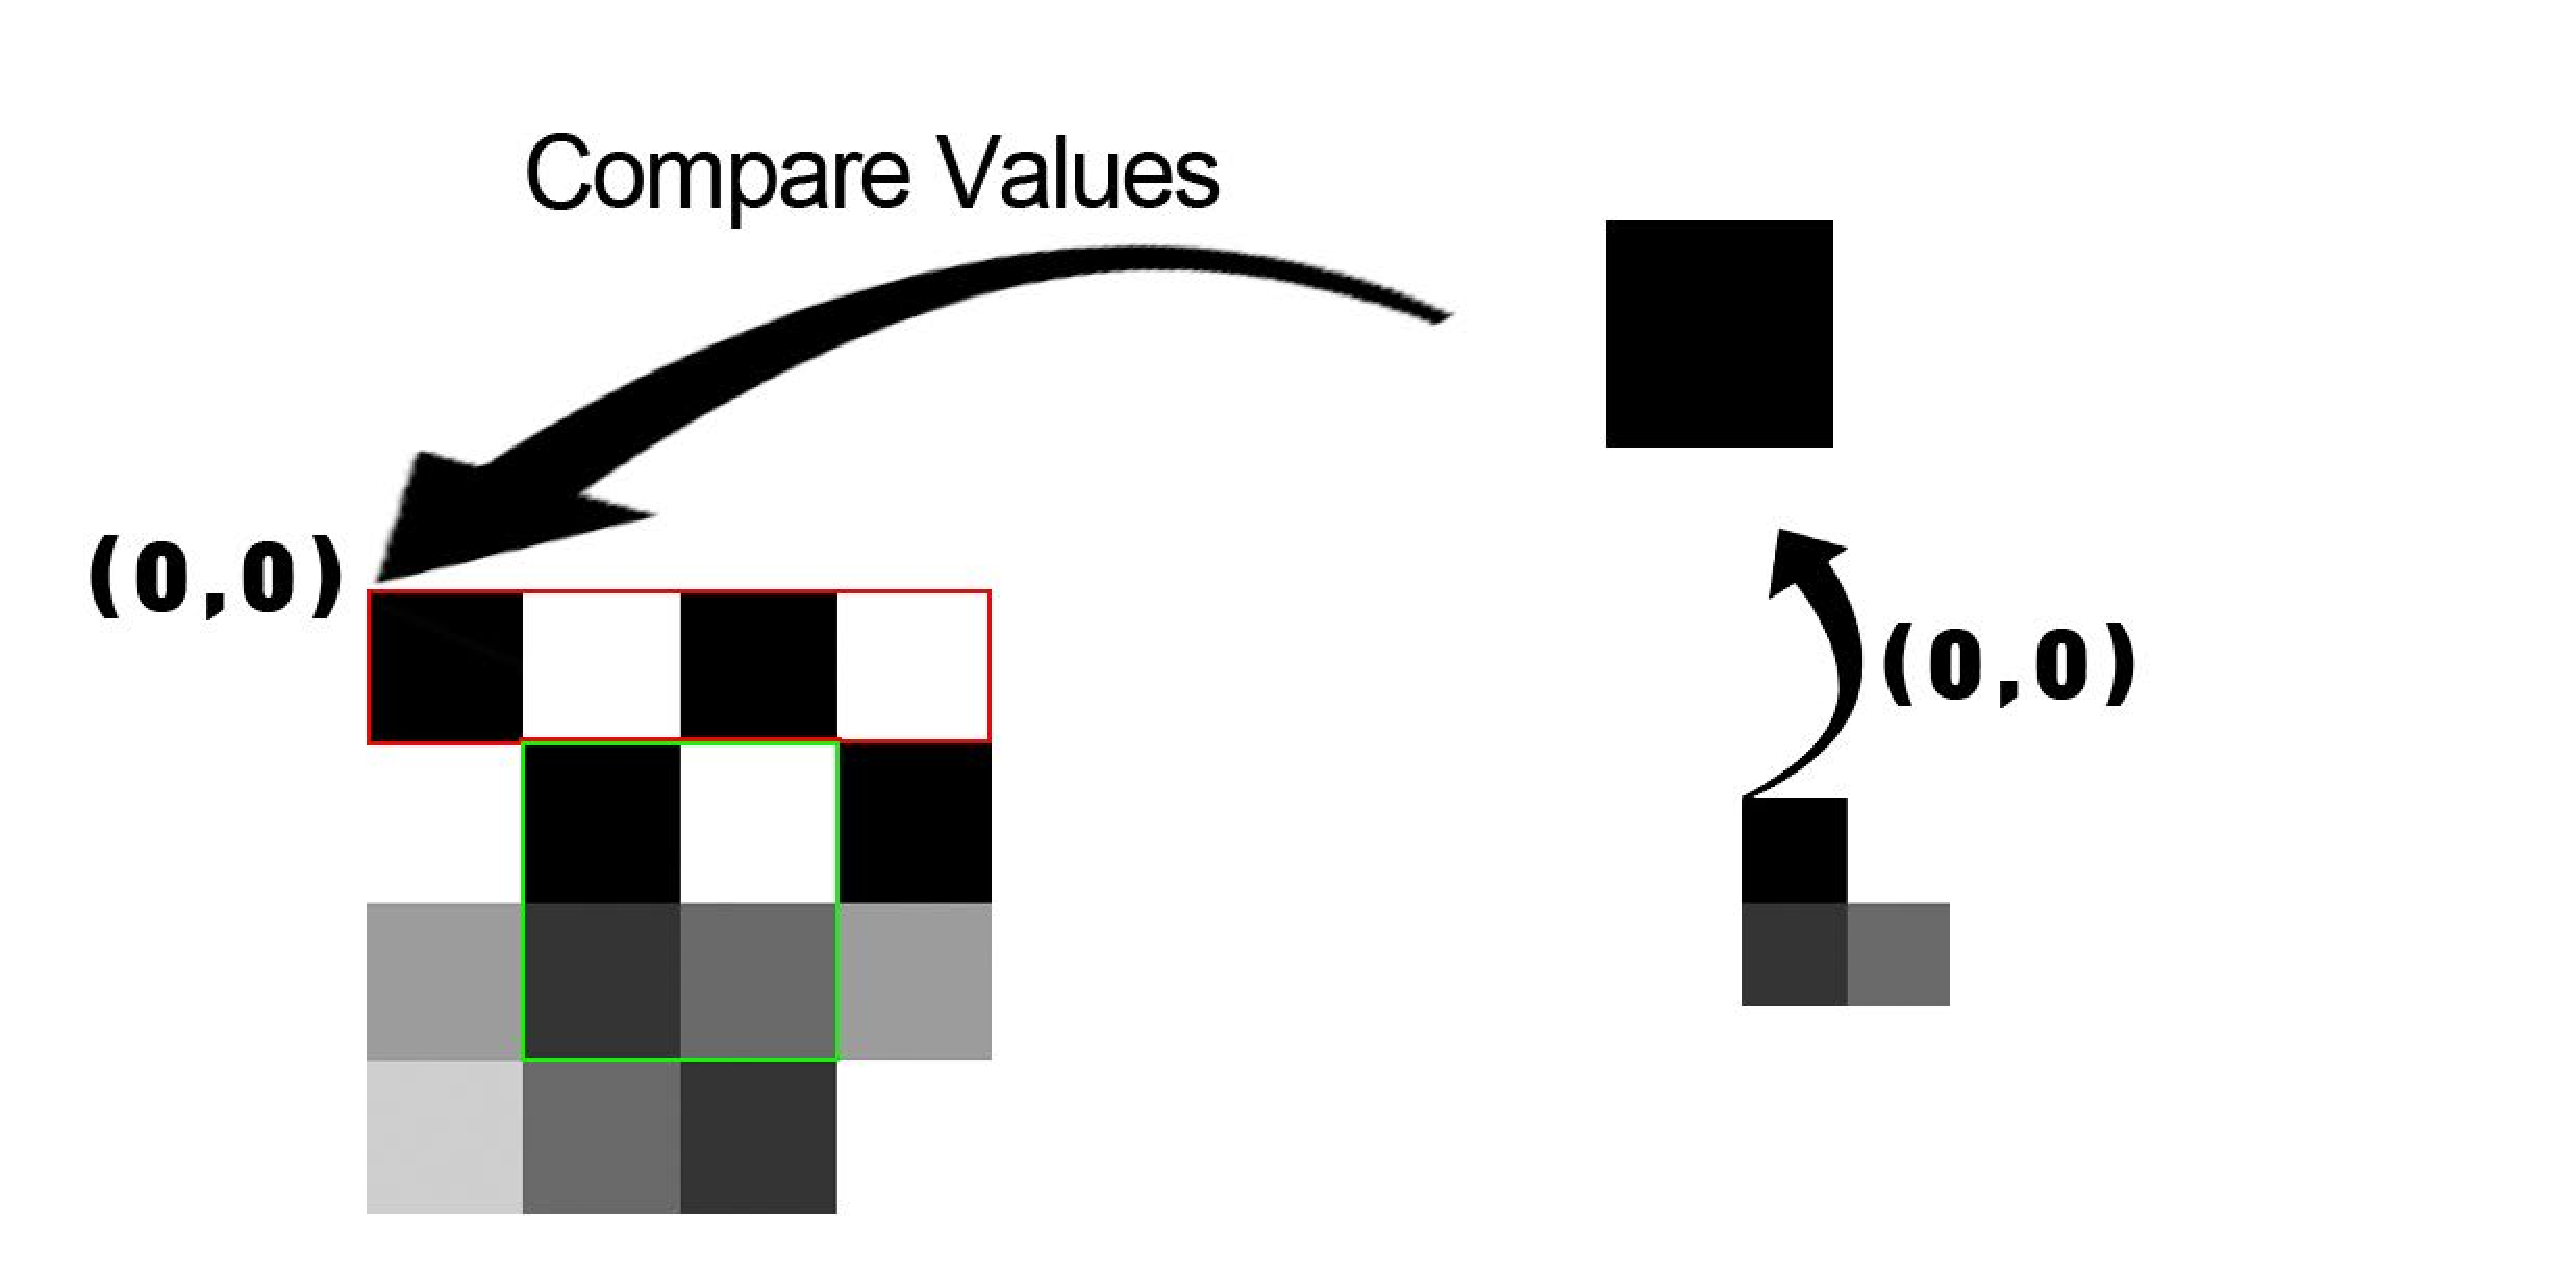
\includegraphics[scale=0.25]{images/Locate_Function.pdf}
        \caption{Figura 1: Figura representativa do funcionamento da ImageLocateSubImage()}
        \label{fig:locate}
    \end{figure}

    \par Após detetar um valor igual ao primeiro píxel da img2 na img1, é ainda comparado os restantes píxeis para 
        garantir que são iguais, podendo afirmar que img2 é, de facto, uma subimagem da img1. Para fazer essa 
        comparação é usado o seguinte excerto de código, onde i e j são, respetivamente, as coordenadas x e y da 
        img2, e são comparados os pixeis equivalentes. Para isso é adicionado ao i e j as coordenadas da img1, caso
        estejamos a localizar a img2 no ponto (x,y) que não seja (0,0) da img1.

    \begin{lstlisting}
        for(int j =0;j < img2->height;j++) {
            for(int i = 0;i < img2->width;i++) {
              if (ImageGetPixel(img1,x + i ,y + j) != ImageGetPixel(img2, i, j)) {
                return 0}
            }
        }
    \end{lstlisting}
